\documentclass[10pt,twocolumn,letterpaper]{article}
\usepackage[margin=0.7in,columnsep=0.25in]{geometry}
\usepackage{amsmath,amssymb,graphicx,booktabs,caption}
\makeatletter\newcommand\tabinput[1]{\@@input #1 }\makeatother
\usepackage[numbers,sort&compress]{natbib}
\captionsetup{font=small,labelfont=bf}
\setlength{\parskip}{0pt}
\makeatletter\renewcommand\section{\@startsection{section}{1}{0pt}{-7pt}{2pt}{\normalfont\large\bfseries}}\makeatother
\title{\vspace{-0.6in}\Large Do Pantheon+ supernovae allow a $\Lambda=0$ dust universe with a lump toward the CoE?}
\author{Note for Chris, \today}
\date{\vspace{-0.35in}}
\begin{document}
\maketitle

\section{Question}
Your programme explains the Migkas et al.\ \cite{Migkas2020,Migkas2021} cluster anisotropy with ordinary gravity from a large mass concentration toward the centre of expansion (CoE), with no dark energy and no dark matter. The previous note showed that the exact relativistic version of that geometry gives the right size, shape, axis and sign for the nearby cluster signal. Here we ask whether the same geometry survives the Pantheon+ type Ia supernova (SN) Hubble diagram \cite{Scolnic2022,Brout2022}, which covers the whole sky out to high redshift and is the data set that established cosmic acceleration in the first place. We fit the SNe with exact Lema\^itre--Tolman--Bondi (LTB) dust models with $\Lambda=0$ and compare them with flat $\Lambda$CDM and with open Friedmann models. We also test directly whether the SN residuals show any anisotropy aligned with the CoE.

\section{Models and data}
We use the LTB metric \cite{Bondi1947,Bolejko2011}
\begin{equation}\label{eq:ltb}
\begin{split}ds^2&=-dt^2+\frac{R'^2}{1+2E(r)}\,dr^2+R^2d\Omega^2,\\ \dot R^2&=\frac{2M(r)}{R}+2E(r),\end{split}
\end{equation}
with the solver, bang-time choice and off-centre geodesic code of the previous note. The mass function is an optional uniform background of density parameter $\Omega$ plus your $e^{-r/L}$ lump, and the observer sits at distance $D$ from the lump centre with local expansion rate $H_0$. We label the lump by its mass inside $D$ in units of the critical mass,
\begin{equation}\label{eq:mc}
m_c=\frac{2G\,M_{\rm lump}(<D)}{H_0^2D^3},
\end{equation}
so that your best fit has the values in the first row of Table~\ref{tab:par}. Two backgrounds carry physical meaning for your programme. The first is a baryons-only background, $\Omega=0.05$, which is what a universe without dark matter contains. The second is $\Omega=0.3$, which we call $\Lambda$CDM-equivalent matter because it is the matter density that $\Lambda$CDM needs, most of it dark. We also let $\Omega$ float. For each geometry we tabulate the luminosity distance $D_L(z,\psi)$ on Gauss--Legendre nodes in the angle $\psi$ from the lump axis and interpolate to every SN direction.

The data are the Pantheon+ corrected magnitudes $m_{b,\rm corr}$ with the full statistical plus systematic covariance $\mathbf C$, using the peculiar-velocity-corrected redshift $z_{\rm HD}$. Our baseline cut is $z>0.023$, and we repeat the main fits with $z>0.01$. The absolute magnitude and $H_0$ enter only as one additive offset $\mathcal M$, which we remove analytically,
\begin{equation}\label{eq:chi2}
\chi^2=\mathbf r^{\sf T}\mathbf C^{-1}\mathbf r-\frac{(\mathbf 1^{\sf T}\mathbf C^{-1}\mathbf r)^2}{\mathbf 1^{\sf T}\mathbf C^{-1}\mathbf 1},\qquad \mathbf r=\mathbf m_{b,\rm corr}-\boldsymbol\mu_{\rm model}.
\end{equation}
To compare models with different numbers of parameters $k$ (the offset included) over $N$ SNe we quote
\begin{equation}\label{eq:ic}
{\rm AIC}=\chi^2+2k,\qquad {\rm BIC}=\chi^2+k\ln N .
\end{equation}
For the fully free LTB model we count seven parameters ($D$, $L$, $M$, $\Omega$, the axis $\ell_0,b_0$, and the offset), even though some are degenerate (Sec.~\ref{sec:fits}), which is conservative.

\section{Fits}\label{sec:fits}
Table~\ref{tab:fits} lists the results and Table~\ref{tab:par} the geometries. Flat $\Lambda$CDM is the reference. Every $\Lambda=0$ dust model is far behind it. The best open Friedmann models are Milne and the baryons-only open universe, and the best free LTB model improves on Milne only slightly while using six extra parameters, so it is no better once the information criteria are applied. This free LTB fit is itself nearly empty and nearly homogeneous, with a small low-mass lump whose axis is far from the CoE.

Your exact geometry, with the axis fixed at the CoE and no background, is much worse than Milne. Adding a baryons-only background helps a lot, and letting $\Omega$ float returns a value close to the baryon density, so a universe without dark matter is what the SNe prefer among these models. Adding $\Lambda$CDM-equivalent matter makes the fit worse and also makes the universe younger than the oldest stars. Freeing the axis improves each case, but the preferred axes move away from the CoE, toward the Galactic poles, where the lump mainly shifts the overall distance scale.

Two degeneracies control the free fits. At fixed $m_c$ and $L/D$ the $\chi^2$ hardly depends on $D$, because the tidal field at the observer scales as $GM/D^3\propto m_cH_0^2$, and the SNe measure only that combination. The background $\Omega$ is pushed to its lower bound whenever the lump is free, because every unit of matter decelerates the expansion and the SNe want acceleration. The deficit relative to $\Lambda$CDM therefore comes from the monopole, the average $D_L(z)$ over the sky, and not from the direction dependence. Figure~\ref{fig:hub} shows this. In all three direction bins the data follow $\Lambda$CDM within the binned errors, the open models sit above it at low $z$ and below it near $z\sim0.5$, and your geometry adds a quadrupole of the size predicted for the clusters, pulling the toward- and away-from-CoE bins down relative to the perpendicular bin. The data show no such quadrupole.

\begin{table*}[t]\centering\footnotesize
\caption{Pantheon+ fits for $z_{\rm HD}>0.023$. $k$ counts the free parameters, the offset included. Differences are with respect to flat $\Lambda$CDM. The column $\Delta\chi^2_{0.01}$ repeats the fit for $z_{\rm HD}>0.01$ where it was done. $t_0$ is the age for $H_0=70$ and $73$ km\,s$^{-1}$\,Mpc$^{-1}$. ``Joint'' rows are the geometries that minimise $\chi^2_{\rm SN}+\chi^2_{\rm cl}$ (Sec.~\ref{sec:mig}), and their $\chi^2$ is the SN part only. The sample size $N$ is given in Table~\ref{tab:dip}.}\label{tab:fits}
\begin{tabular}{@{}lrrrrrrrr@{}}\toprule
Model & $k$ & $\chi^2$ & $\Delta\chi^2$ & $\Delta$AIC & $\Delta$BIC & $\Delta\chi^2_{0.01}$ & $t_0^{(70)}$ [Gyr] & $t_0^{(73)}$ [Gyr]\\\midrule
\tabinput{tab_fits.tex}
\bottomrule\end{tabular}\end{table*}

\begin{table*}[t]\centering\footnotesize
\caption{LTB geometries. $D$ is in the geometric units of the previous note, $m_c$ follows Eq.~(\ref{eq:mc}), $(\ell_0,b_0)$ is the lump axis, $\theta_{\rm CoE}$ its angle from the CoE, and $\chi^2$ the SN value for $z_{\rm HD}>0.023$.}\label{tab:par}
\setlength{\tabcolsep}{2.5pt}
\begin{tabular}{@{}lrrrrrrrr@{}}\toprule
Geometry & $D$ & $L/D$ & $m_c$ & $\Omega$ & $\ell_0$ & $b_0$ & $\theta_{\rm CoE}$ & $\chi^2$\\\midrule
\tabinput{tab_par.tex}
\bottomrule\end{tabular}\end{table*}

\begin{figure*}[t]\centering
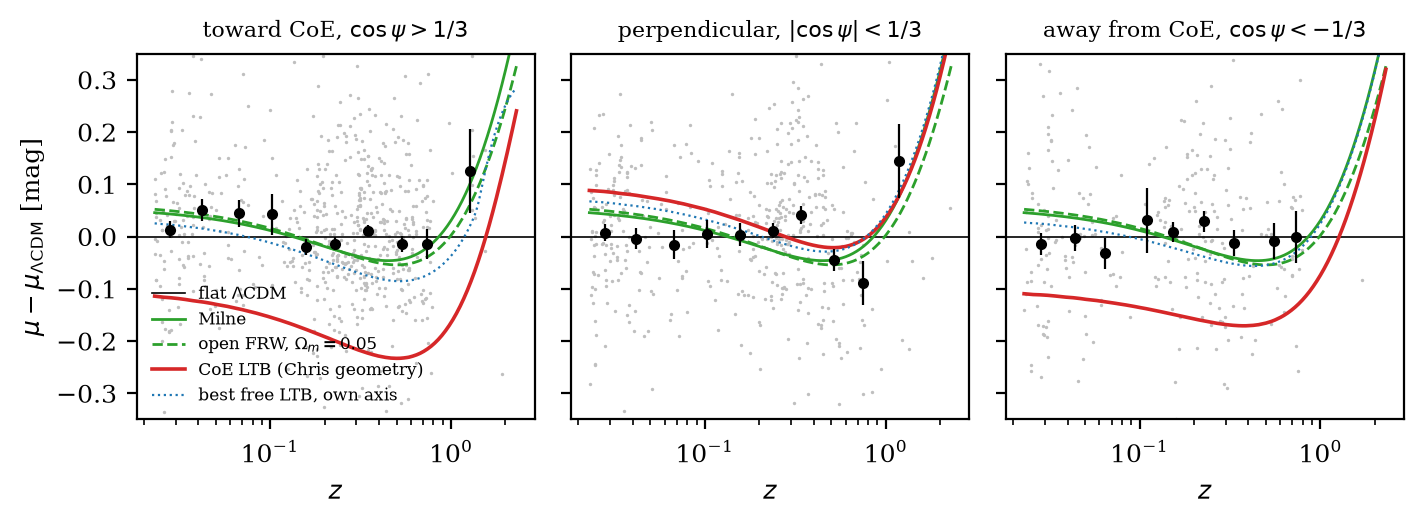
\includegraphics[width=\textwidth]{fig_hubble_resid.png}
\caption{Pantheon+ distance moduli relative to flat $\Lambda$CDM, split by the angle $\psi$ between each SN and the CoE. Grey points are individual SNe and black points are inverse-variance binned means with diagonal errors, for display only. The curves are Milne (solid green), the baryons-only open universe (dashed green), your CoE geometry evaluated along the bin's central direction (red), and the best free LTB model along its own axis (dotted blue). Each model uses its own best-fit offset.}\label{fig:hub}
\end{figure*}

\section{Direction tests}
We also looked for anisotropy in the SN residuals without assuming a model. We fit a dipole to the residuals from each model with the full covariance,
\begin{equation}\label{eq:dip}
m_{b,{\rm corr},i}-\mu_{\rm model}(z_i)=\mathcal M+\mathbf d\cdot\hat{\mathbf n}_i ,
\end{equation}
and we repeat the redshift-dependent deceleration test of Colin et al.\ \cite{Colin2019},
\begin{equation}\label{eq:colin}
q_0(\hat{\mathbf n})=q_m+q_d\,(\hat{\mathbf n}\cdot\hat{\mathbf c})\,e^{-z/S},\qquad S=0.0262,
\end{equation}
together with a simple split into hemispheres. Tables~\ref{tab:dip} and~\ref{tab:q} give the results, and Fig.~\ref{fig:sky} shows the residual map.

The only residual dipole with modest significance is in the lowest redshift bin, and its axis lies between the CoE and the Galactic anticentre direction. The higher redshift bins show nothing coherent. With the Colin parametrisation, a CMB-dipole axis gives a positive $q_d$, the Migkas axis gives nothing, and the CoE axis gives a negative $q_d$, meaning faster apparent acceleration toward the CoE. None of these is significant, and the sign found by Colin et al.\ is not reproduced once Pantheon+ uses corrected redshifts. The hemisphere values agree within their errors for every axis. The low-$z$ dipole is also the regime most sensitive to the flow model behind $z_{\rm HD}$, so we treat it as a hint and not as a detection. Its axis is closer to the CoE than to any other tested axis, but the LTB lump produces mainly a quadrupole, so this alignment is not a prediction of the model, and the free LTB fits do not turn it into a better global fit.

\begin{table*}[t]\centering\footnotesize
\caption{Residual dipoles from Eq.~(\ref{eq:dip}) with the full covariance. $A$ is the dipole amplitude in magnitudes (positive means more distant than the model), $\delta\theta_{68}$ the 68\% direction uncertainty, $\theta_{\rm CoE}$ the angle from the CoE, and $\Delta\chi^2$ the improvement over no dipole for three extra parameters.}\label{tab:dip}
\setlength{\tabcolsep}{2.2pt}
\begin{tabular}{@{}lrrrrrrrr@{}}\toprule
Residuals & $N$ & $A$ & $\sigma_A$ & $\ell$ & $b$ & $\delta\theta_{68}$ & $\theta_{\rm CoE}$ & $\Delta\chi^2$\\\midrule
\tabinput{tab_dip.tex}
\bottomrule\end{tabular}\end{table*}

\begin{table*}[t]\centering\footnotesize
\caption{Deceleration-parameter anisotropy from the cosmographic expansion with $z<0.8$. Columns 3--6 are the fit of Eq.~(\ref{eq:colin}) with $j_0$ free, and $\Delta\chi^2$ is its improvement over $q_d=0$. The last four columns give $q_0$ with $j_0=1$ in the hemisphere toward the axis and in the opposite one. The last axis is the $\Lambda$CDM residual dipole of Table~\ref{tab:dip}, so its $\Delta\chi^2$ carries a look-elsewhere penalty.}\label{tab:q}
\setlength{\tabcolsep}{1.6pt}
\begin{tabular}{@{}llrrrrrrrr@{}}\toprule
$z_{\rm min}$ & Axis & $q_m$ & $q_d$ & $\sigma_{q_d}$ & $\Delta\chi^2$ & $q_0^{\rm tow}$ & $\sigma$ & $q_0^{\rm away}$ & $\sigma$\\\midrule
\tabinput{tab_q.tex}
\bottomrule\end{tabular}\end{table*}

\begin{figure*}[t]\centering
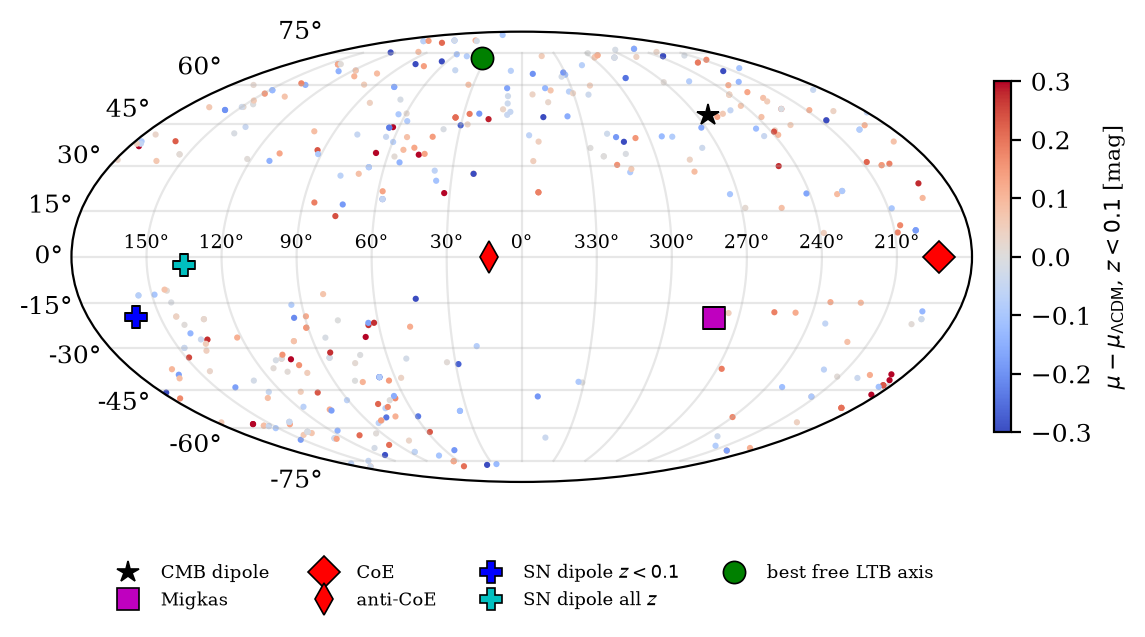
\includegraphics[width=0.72\textwidth]{fig_sky.png}
\caption{Galactic Mollweide map (longitude increasing to the left) of $\Lambda$CDM residuals for $z_{\rm HD}<0.1$, with the CMB dipole (also the axis tested by Colin et al.\ \cite{Colin2019}), the Migkas cluster axis, the CoE and anti-CoE, the $\Lambda$CDM residual dipoles, and the best free LTB axis.}\label{fig:sky}
\end{figure*}

\section{Consistency with the cluster anisotropy}\label{sec:mig}
In Migkas's convention the cluster normalisation scales as $A\propto H_0^2$, so we model it as
\begin{equation}\label{eq:A}
\frac{A(\ell)}{\langle A\rangle}=\frac{D_L^{-2}(z=0.1,\ell,b=0)}{\big\langle D_L^{-2}\big\rangle}
\end{equation}
and compare with the digitised $A(\ell)$ profile, using a free normalisation and diagonal errors. Table~\ref{tab:mig} gives the results. Your geometry with the CoE axis improves strongly on isotropy and follows the data closely. The SN-preferred geometries give essentially no cluster signal, and your lump rotated to the SN-preferred axis is ruled out by the clusters. A joint fit of both data sets over $L/D$, $m_c$ and the axis lands close to the CoE, slightly below the Galactic plane, with a lump broader and slightly lighter than yours. It keeps most of the cluster improvement and costs the SNe very little relative to the best $\Lambda=0$ models. So the SN data do not exclude a lump toward the CoE. What they exclude is the $\Lambda=0$ dust monopole, whatever lump is added.

The cluster $\chi^2$ values overstate the evidence, because the digitised points come from overlapping sliding cones and are strongly correlated. The comparison between rows is more reliable than the absolute numbers.

\begin{table}[t]\centering\footnotesize
\caption{Cluster anisotropy test with Eq.~(\ref{eq:A}) at $z=0.1$ along $b=0$, using the digitised Migkas $A(\ell)$ profile. The $\chi^2_{\rm cl}$ values use diagonal errors on correlated points (see text). $r$ is the Pearson correlation between model and data, and the last two columns give the SN $\chi^2$ of the same geometry and its offset from $\Lambda$CDM.}\label{tab:mig}
\setlength{\tabcolsep}{2.5pt}
\begin{tabular}{@{}lrrrr@{}}\toprule
Geometry & $\chi^2_{\rm cl}$ & $r$ & $\chi^2_{\rm SN}$ & $\Delta\chi^2_{\rm SN}$\\\midrule
\tabinput{tab_mig.tex}
\bottomrule\end{tabular}\end{table}

\section{Ages}
All $\Lambda=0$ models without dark matter have ages comparable to the oldest globular clusters, which are 12--13 Gyr old, when $H_0=70$. Adding $\Lambda$CDM-equivalent matter, or using $H_0=73$, pushes the lump models below that range (Table~\ref{tab:fits}). The age is therefore not a strong discriminant for the baryons-only models, and it counts against the model with $\Lambda$CDM-equivalent matter.

\section{Caveats}
The $z_{\rm HD}$ redshifts include peculiar-velocity corrections computed from a flow model built in $\Lambda$CDM, and those corrections contain part of the nearby anisotropy we are testing. The low-$z$ dipole and the cluster comparison are the parts most affected, while the high-redshift monopole deficit is not. The Pantheon+ standardisation and systematics were built in a $\Lambda$CDM framework. We model dust only, with $\Lambda=0$, so radiation, pressure and any late-time physics outside LTB are absent. The cluster profile is a digitised figure with correlated points, and we use only the $b=0$ ring. The free-LTB search used several Nelder--Mead starts on a nearly flat surface, so its optimum is shallow, although the conclusion does not depend on its exact location.

\section{Conclusion}
The Pantheon+ Hubble diagram does not care where the lump is. It rejects any $\Lambda=0$ dust universe, with or without a CoE lump, by a wide margin relative to flat $\Lambda$CDM (Table~\ref{tab:fits}), and the rejection comes from the sky-averaged distance--redshift relation. Within the $\Lambda=0$ family the SNe prefer a universe without dark matter, a baryons-only or emptier background, which is consistent with your programme. The directional information is neutral to mildly favourable: the only residual dipole, at low redshift, lies closer to the CoE than to the other tested axes, and a lump near the CoE that fits the clusters costs the SNe little compared with Milne. The open problem for the programme is the monopole, meaning the apparent acceleration seen by distant SNe, and adding the lump that the clusters need does not supply it.

\begin{thebibliography}{99}\footnotesize
\bibitem{Migkas2020} K.~Migkas et al., A\&A 636, A15 (2020).
\bibitem{Migkas2021} K.~Migkas et al., A\&A 649, A151 (2021).
\bibitem{Scolnic2022} D.~Scolnic et al., ApJ 938, 113 (2022).
\bibitem{Brout2022} D.~Brout et al., ApJ 938, 110 (2022).
\bibitem{Bondi1947} H.~Bondi, MNRAS 107, 410 (1947).
\bibitem{Bolejko2011} K.~Bolejko, M.-N.~C\'el\'erier, A.~Krasi\'nski, Class.\ Quantum Grav.\ 28, 164002 (2011).
\bibitem{Colin2019} J.~Colin, R.~Mohayaee, M.~Rameez, S.~Sarkar, A\&A 631, L13 (2019).
\end{thebibliography}
\end{document}
